%
% Copyright (c) 2017-2018  Maximilian Wuttke
%

% BUGS
% - https://tex.stackexchange.com/questions/9633/why-should-i-put-a-before-ref-or-cite

\documentclass{psartcl}
%%%
%%% Shared preamble for all files, e.g. thesis, TikZ standalones, slides, etc.
%%% It defines \macros for types, Turing machines, etc.
%%%

% Packages needed
\usepackage[utf8]{inputenc}
\usepackage{geometry}
\usepackage[small,compact]{titlesec}
\usepackage[final]{listings}
\usepackage{amsmath}
\usepackage[amsmath,hyperref,thmmarks]{ntheorem}
% Warning: The package ntheorem defines a \None macro!
\usepackage{amssymb}
\usepackage{tipa}
\usepackage[english]{babel}
\usepackage{lstautogobble}
\usepackage{proof}
\usepackage{bussproofs}
\usepackage{xparse}
\usepackage{needspace}
\usepackage{xspace}
\usepackage{mathpartir}
\usepackage{stmaryrd} % for |llbracket and \rrbracket
\usepackage{standalone} % useful to out-source graphics


% TikZ ist *kein* Zeichenprogramm.
\usepackage{tikz}
\usetikzlibrary{arrows,shapes,snakes,automata,backgrounds,fit,positioning}
\usepackage{tikz-cd} % for commutative diagrams


%% Formating
\newcommand{\MS}[1]{\ensuremath{\mathsf{#1}}}
\newcommand{\MST}[1]{${\mathsf{#1}}$}
\newcommand{\IsMathMode}{\ifmmode{This is math mode}\else{This is not math mode}\fi}

%% Logic symbols
\newcommand{\defop}{\mathop{:=}}
\newcommand{\imp}{\mathbin{\rightarrow}~}
\newcommand{\Imp}{\mathbin{\Rightarrow}~}
\renewcommand{\iff}{\mathbin{\leftrightarrow}}


% ++ operator:
% Source: https://tex.stackexchange.com/questions/4194/how-to-typeset-haskell-operator-and-friends
\newcommand\doubleplus{+\kern-1.3ex+\kern0.8ex}
\newcommand\mdoubleplus{\ensuremath{\mathbin{+\mkern-10mu+}}}
\newcommand{\app}{\mdoubleplus}

\newcommand{\rew}{\Rightarrow}
\newcommand{\trew}{\stackrel{\textrm{T}}\Rightarrow}
\newcommand{\llrew}{\stackrel{\textrm{L}}\Rightarrow}
\newcommand{\rlrew}{\stackrel{\textrm{R}}\Rightarrow}
\newcommand{\arew}{\triangleright}
\newcommand{\conc}{\mathop{{+}\hskip-5pt{+}}}
\newcommand{\gen}{\Rightarrow}

%% Sets
% \newcommand{\lam}[2]{\lambda#1{.}\hskip.7pt#2}
\newcommand{\setOf}[1]{\bigl\{ #1 \bigr \}}
\newcommand{\setMap}[2]{\setOf{#1~\big|~#2}}
\newcommand{\depPair}[2]{\setOf{#1~{\&}~#2}}
\newcommand{\pair}[2]{\bigl( #1 , #2 \bigr)}
\newcommand{\class}[1]{\bigl[ #1 \bigr]}
\newcommand{\choice}[1]{\bigl< #1 \bigr>}
\newcommand{\explainRel}[2]{\stackrel{\text{#1}}{#2}}
\newcommand{\family}[2]{\bigl( #1 \bigr)_{#2}}
\newcommand{\from}{:}
\renewcommand{\to}{\rightarrow}

%% Types
\newcommand{\Bool}{\mathbb{B}}
\newcommand{\Fin}{\mathbb{F}}
\newcommand{\Nat}{\mathbb{N}}
\newcommand{\Prop}{\mathbb{P}}
\newcommand{\Type}{\mathbb{T}}
\newcommand{\Unit}{\MS{1}}
\newcommand{\Option}{\mathcal{O}}
\newcommand{\List}{\mathcal{L}}
\newcommand{\Rel}{\MS{Rel}}

\newcommand{\True}{\top}
\newcommand{\False}{\bot}

%% Tapes
\newcommand{\tape}[1]{[ #1 ]}
\newcommand{\tapePointer}[1]{\underset{\uparrow}{#1}}
\newcommand{\niltape}{\tape{\tapePointer{}}}
\newcommand{\midtape}[3]{\tape{#1~\tapePointer{#2}~#3}}
\newcommand{\leftof}[2]{\tape{\tapePointer{}~#1~#2}}
\newcommand{\rightof}[2]{\tape{#1~#2~\tapePointer{}}}

% \newcommand{\niltape}{\MS{niltape}}
% \newcommand{\midtape}[3]{\MS{midtape}~#1~#2~#3}
% \newcommand{\leftof}[2]{\MS{leftof}~#1~#2}
% \newcommand{\rightof}[2]{\MS{rightof}~#1~#2}

%% Turing machine types
\newcommand{\Loop}{\MS{loop}}
\newcommand{\Tape}{\MS{Tape}}
\newcommand{\Tapes}[1]{\Tape^{#1}}
\newcommand{\TM}{\MS{TM}}
\newcommand{\Move}{\MS{Move}}
\newcommand{\Act}{\MS{Act}}
\newcommand{\Conf}{\MS{Conf}}
\newcommand{\Tau}{\Gamma}

%% Relations
\newcommand{\rif}{\mathbin{\phi}}
\newcommand{\at} [2][]{#1{|}_{#2}}
\newcommand{\att}[2][]{#1{|\mkern-1.5mu|}_{#2}}
\DeclareMathOperator{\ignoreParam}{\Uparrow}
\DeclareMathOperator{\hideParam}{\Downarrow}


%% Constructors
\DeclareMathOperator{\inl}{\ensuremath{\MS{inl}}}
\DeclareMathOperator{\inr}{\ensuremath{\MS{inr}}}
\newcommand{\Some}[1]{\left\lfloor {#1} \right\rfloor}
% \None is defined sometimes
\renewcommand{\None}{\emptyset}
\newcommand{\true}{\MS{true}}
\newcommand{\false}{\MS{false}}
\newcommand{\unit}{\MS{()}}
\newcommand{\nil}{\MS{nil}}
\newcommand{\cons}{\mathbin{::}}

%% Functions
\newcommand{\map}[2]{\ensuremath{\MS{map}~#1~#2}}
\newcommand{\maptwo}[3]{\ensuremath{\MS{map}_2~#1~#2~#3}}
\newcommand{\rev}[1]{\MS{rev}~#1}

%% Vector
\newcommand{\Vector}[1]{\left[ #1 \right]}
\DeclareMathOperator{\hd}{\ensuremath{\MS{hd}}}
\DeclareMathOperator{\tl}{\ensuremath{\MS{tl}}}
\newcommand{\length}[1]{\left| #1 \right|}
\newcommand{\blength}[1]{\bigl| #1 \bigr|}


%%
%% Encding
%%
\newcommand{\contains}{\simeq}
\newcommand{\size}[1]{\length{encode(#1)}}

%% Semantics
\newcommand{\terminates}{\mathrel{\triangleright}}
\newcommand{\TerminatesIn}{\mathrel{\downarrow}}
\newcommand{\Realise}{\mathrel{\vDash}}
\newcommand{\RealiseIn}[1]{\mathrel{\vDash^{#1}}}

%%
%% Turing Machines
%%

%% Control flow operators
\newcommand{\While}{\MS{While}}
\newcommand{\Seq}{;~}
\newcommand{\Match}{\MS{Match}}
\newcommand{\If}[3]{\MS{If}~#1~\MS{Then}~#2~\MS{Else}~#3}
\newcommand{\Let}[2]{\MS{let}~#1~\MS{in}~#2}
\newcommand{\cond}[3]{\MS{if}~#1~\MS{then}~#2~\MS{else}~#3}
\newcommand{\Nop}{\MS{Nop}}
\newcommand{\Return}[2]{\MS{Return}~#1~#2}
% \newcommand{\Return}[2]{\MS{Return}_{#2}~#1}

%% Lifts
% #1 is the machine, #2 the lifting
\newcommand{\LiftTapes}[2]{\mathop{\Uparrow_{#2}} #1}
\newcommand{\LiftAlphabet}[2]{\mathop{\Uparrow_{#2}} #1}
% #1 is the machine, #2 the alphabet lifting, and #3 the tape-lifting
\newcommand{\LiftBoth}[3]{\mathop{\Uparrow_{#2;~#3}} #1}




%%%
%%% lstlisting
%%%

% Style and language to define complex multi-line definitions similar to Coq code
\lstdefinelanguage{semicoq}{
  keywords={if,then,else,true,false,match,Match,If,Then,Else,Nop,Return,Move,Reset,DoAct,WriteMove,L,R,N},
  comment=[s]{(*}{*)},
}

%% Overlap #2 over phantom #1, e.g.
%% % XX\phalign{abcdefg}{YY}XX \\
%% % XXabcdefgXX
%% gets
%% XXYY     XX
%% XXabcdefgXX
%% Idea from https://tex.stackexchange.com/questions/212710/fill-space-created-by-phantom-with-other-text
\newcommand{\phalign}[2]{\makebox[0pt][l]{\ensuremath{#2}}\phantom{#1}}

\lstdefinestyle{semicoqstyle}{
  mathescape=true,
  keywordstyle=\textsf,
  language=semicoq,
  literate={
    {=>}{{$\Rightarrow$}}2
    {>->}{{$\rightarrowtail\,$}}2
    {<->}{{$\leftrightarrow$ }}2
    {->}{{$\to$ }}3
    {~}{{$\lnot$}}1
    {/\\}{{$\land$}}2
    {\\/}{{$\lor$}}2
    {forall}{{$\forall$}}1
    {exists}{{$\exists$}}1
    {<>}{{$\not =$}}{1}
    {<=}{{$\leq$}}{1}
    {<}{{$\lt$}}{1}
    {>=}{{$\ge$}}{1}
    {>}{{$\gt$}}{1}
    {[}{{$[$}}{1}
    {|}{{$|$}}{1}
    {]}{{$]$}}{1}
    {])}{{$])$}}{2}
    {(}{{$($}}{1}
    {)}{{$)$}}{1}
    {match}{{$\MS{match}$}}5
    {if}{{$\MS{if}$}}1
    {then}{{$\phalign{\MS{else}}{{\MS{then}}}$}}3
    {else}{{$\phalign{\MS{else}}{{\MS{else}}}$}}3
    {If}{{$\MS{If}$}}2
    {Then}{{$\phalign{\MS{Else}}{{\MS{Then}}}$}}4
    {Else}{{$\phalign{\MS{Else}}{{\MS{Else}}}$}}4
  }
}

\lstdefinelanguage{pseudocode}{
  keywords={If,Then,Else,Do,While,Reset,Return,Continue,Break},
}

\lstdefinestyle{pseudocode}{
  mathescape=true,
  language=pseudocode,
  literate={
    {:=}{{$\leftarrow$}}{2}
    {<>}{{$\not =$}}{1}
    {<=}{{$\leq$}}{1}
    {<}{{$\lt$}}{1}
    {>=}{{$\ge$}}{1}
    {>}{{$\gt$}}{1}
  }
}






%%% Local Variables:
%%% mode: LaTeX
%%% TeX-master: "thesis"
%%% End:

\begin{document}

\title{A Formalisation Of Multi-Tape \\ Turing Machines In Coq}
\author{Maximilian Wuttke}
\date{Saarland University\\\today}
\maketitle

\begin{abstract}
  Developing and verifying Turing machines can be a tedious task because they are very low level.  Turing machines can be completely unstructured:
  from any state of the execution, it could continue at any other state.  Furthermore Turing machines are not compositional: Having two Turing
  machines $A$ and $B$ it is not trivial to generate a new machine $A \mseq B$ that executes a copy of $B$ after the execution of a copy of $A$.
  Control flow operations, like if then else and while have to be constructed and verified first.  However, it is also not clear how to combine
  machines with different alphabets and numbers of tapes.

  We carried over the basic definition of multi-tape Turing machines from the Matita devolepment of Asperti et al.  Our aproach for defining the
  semantics of machine is similiar to the aproach choosen by Asperti et al.  We define specifications for Turing machines in terms of relations over
  tape vectors.  Relations have the benefit of being compositional.  For example, the correctness statement of our $\MS{While}$ operator can be
  expressed using the relational Kleene star operator.  Our new aproach makes it superfluent to reason about internal states of machines.  We also
  show how to reason about runtime and space usage.

  The first contribution of this thesis is a framework devoleped in Coq, for programming and verifying multi-tape Turing machines.  Secondly, we use
  this framework to implement and verify an interpreter for the weak call-by-value $\lambda$-calculus.
\end{abstract}



\section{Notations}
In this memo, I use bold font to denote the constants: $\true$, $\false$, and $\unit$.  Types are written in sans-serif font and capitalized: $\Type$,
$\Prop$, $\Rel(X, Y)$, $\Unit$, $\Bool$, $\Nat$, and $\Option$.  We use the infix operator $+$ to denote sum-types.  $\Some{\cdot}$ and $\None$ denote
the values of the option type $\Option(\cdot)$.  For record types $R$, $x_{(\cdot)}$ denotes the projection function of the member $x$ of $R$.
$(f, g) \from X \hookrightarrow Y$ denotes either a retract from $X$ to $Y$ and $f \from X \hookrightarrow Y$ a injection from $X$ to $Y$.
Later we will also write $X \hookrightarrow Y$ to denote the canonical (tight) retract or injection from $X$ to $Y$, if we have defined it before and
if it is clear weather we mean the retract or the injection.  (This is analogous in the Coq-development:  Since we use type-classes there, we often
do not have to specify those functions since they can be inferred automatically.)  Set-notations are used to define relations.

Vectors and lists are $0$-indexed.  We write numbers $n < k$ when we mean values of the finite Type $\Fin_k$, where $k\in\Nat$.

\section{Definition of multi-tape Turing machines}
\label{sec:def}

\begin{definition}[Multi-tape Turing machine]
  \label{def:mTM}
  There are three possible movements:  $\MS{Move} := \setOf{L, R, N}$.
  An \emph{$n$-tape Turing machine} over a finite alphabet $\Sigma$ is a record $M = (Q, \gamma, s, h)$ where
  \begin{itemize}
    \item $Q$ is the finite type of states,
    \item $\gamma \from Q \times (\Option~\Sigma)^n \to Q \times (\Option~\Sigma \times \MS{Move})^n$ is the transition function that for every state and
      vector of $n$ read symbols yields the new state and a vector of $n$ symbols to write and a direction to move,
    \item $s:Q$ is the start state,
    \item $h \from Q \to \Bool$ is the decidable subset of halting states.
  \end{itemize}

  Tuples of the type $\Option(\Sigma) \times \Move$ are called \emph{actions}.  They are refered to with the symbol $\MS{Act}$, if $\Sigma$ is clear.
\end{definition}

At this moment, we make no distinction between input and output tapes.  Note that the transition function has to yield a successor state even on
halting states.  Also note that while we parameterized Definition \ref{def:mTM} over the alphabet $\Sigma$ and the number of tapes $n$, but we
abstract the states.  Our machines behave deterministically, since $\gamma$ is a function.  We write $\MS{TM}_\Sigma^n$ for the type of $n$-tape
Turing machines over the alphabet $\Sigma$.

Later, when we want to verify complex machines, we do not want to reason about internal states.  We rather want to reason about partition of states,
e.g. positive or negative states.  In general, if $F$ is a finite type, then
$\MS{TM}_\Sigma^n(F) := \left\{ M:\MS{TM}_\Sigma^n ~\&~ Q_M \to F \right\}$ is the sigma type of a machine and a partitioning function from the states
to $F$.  For a machine $M$ together with a partition function $p$, we write $(M; p)$.

We also use the definition of \emph{tapes} from the Matita development of Asperti et~al.  Unlike in most mathematical representations, our tapes are
finite.  However, arbitrary much memory can be allocated on the tape.  A tape essentially is a triple $(ls,m,rs)$, where the symbol $m$ is the symbol
on which the (read/write) head of tape is.  Both lists of symbols $ls$ and $rs$ are in the order of the ``distance'' to the head.  However, there are
three cases where there is no current symbol: the tape can be completely empty, or the head can be to the left (or right) outermost of the tape.
Formally, tapes are defined inductively:

\begin{definition}[Tape]
  \label{def:tape}
  Let $\Sigma$ be a finite alphabet.  Then $\Tape_\Sigma$ is defined as the inductive type:
  \begin{align*}
    & \Tape_\Sigma : \Type := \\
    & \quad | \quad \MS{niltape} \\
    & \quad | \quad \MS{leftof}  ~ (r:\Sigma) ~ (rs:\List(\Sigma)) \\
    & \quad | \quad \MS{midtape} ~ (ls:\List(\Sigma)) ~ (m:\Sigma) ~ (rs:\List(\Sigma)) \\
    & \quad | \quad \MS{rightof} ~ (l:\Sigma) ~ (ls:\List(\Sigma)).
  \end{align*}
\end{definition}


We introduce a more informal notation of tapes, where the symbols are represented from left to right.  The position of the head is marked by the
arrow:
\begin{align*}
  \niltape &:= \MS{niltape} ;\\
  \leftof{r}{rs} &:= \MS{leftof}~r~rs ;\\
  \midtape{ls}{m}{rs} &:= \MS{midtape}~(\rev~rs)~m~rs ;\\
  \rightof{ls}{l} &:= \MS{rightof}~(\rev~ls)~l
\end{align*}

Now we can define the \emph{configuration} of a multi-tape Turing machine.  It is captured by the current state and the vector of the $n$ tapes:
\begin{definition}[Configuration]
  \label{def:config}
  A \emph{configuration} of an $n$-tape Turing machine $T$ over the alphabet $\Sigma$ is a record $\MS{Conf} := \{\MS{state}:Q_M; \MS{tapes}:\Tape_\Sigma^n\}$.
\end{definition}

Now we define tape movement and how to write symbols on tapes.  Note that because in the implementation the list of the left side of the pointer is
saved in reversed order, we do not have to execute \MS{app}.  \begin{alignat*}{2}
  \MS{mv}_R&~(\leftof{r}{R}               &&:= \midtape{\nil}{r}{R} \\
  \MS{mv}_R&~(\midtape{L}{m}{\nil})       &&:= \rightof{L}{m} \\
  \MS{mv}_R&~(\midtape{L}{m}{r \cons R)}) &&:= \midtape{L \app [m]}{r}{R} \\
  \MS{mv}_N&~(t)                          &&:= t
\end{alignat*}
The function $\MS{mv}_L$ is defined analogously.
To define the function $\MS{write} \from \Option(\Sigma) \to \Tape \to \Tape$, we first need functions
$\MS{left},~\MS{right} \from \Tape \to \List(\Sigma)$
that return the symbols to the left side of the pointer and respectively the symbols to the right of the pointer.
% TODO: Two collums
\begin{alignat*}{2}
  \MS{left} &~\niltape          &&:= \nil \\
  \MS{left} &~\leftof{r}{R}     &&:= \nil \\
  \MS{left} &~\midtape{L}{m}{R} &&:= L \\
  \MS{left} &~\rightof{L}{l}    &&:= L \app [l] \\
  \MS{right}&~\niltape          &&:= \nil \\
  \MS{right}&~\leftof{r}{R}     &&:= r \cons R \\
  \MS{right}&~\midtape{L}{m}{R} &&:= R \\
  \MS{right}&~\rightof{L}{l}    &&:= \nil
\end{alignat*}
Note that in the implementation $\MS{left}$ returns the same list but again in reserved order, so we do not have to execute $\MS{app}$.
Now we can define $\MS{wr} \from \Tape \to \Option(\Move) \to \Tape$.
When we write $\None$, the tape remains unchanged.
But if we write $\Some a$, we get a $\MS{midtape}$, where the left and right symbols remain unchanged and $a$ is now in the middle.
\begin{alignat*}{3}
  \MS{wr}~t &~ \None   &&:= t \\
  \MS{wr}~t &~ \Some a &&:= \midtape{\MS{left}(t)}{a}{\MS{right}(t)}
\end{alignat*}
To define the function $\MS{step} \from \MS{Conf} \to \MS{Conf}$, we need to know the symbols on the tapes.
Therefore we define a function $\MS{current} \from Tape \to \Option(\Sigma)$.
It returns $\None$ if the pointer is not under a symbol, and $\Some a$ if the pointer is under the symbol $a$.
\begin{alignat*}{2}
  \MS{current}&~(\midtape{L}{m}{R})&&:= \Some m \\
  \MS{current}&~\_                 &&:= \None
\end{alignat*}
We can state a correctness lemma of the function $\MS{write}$:
\begin{lemma}[Write]
  \label{lem:write}
  For all tapes $t$ and symbols $\sigma:\Sigma$:
  % TODO: Align it, for example like in https://tex.stackexchange.com/questions/12771/mix-align-and-enumerate
  \begin{enumerate}
    \item $\MS{right}   (\MS{wr}~t~\Some\sigma) = \MS{right}(t)$
    \item $\MS{left}    (\MS{wr}~t~\Some\sigma) = \MS{left} (t)$
    \item $\MS{current} (\MS{wr}~t~\Some\sigma) = \Some\sigma$
  \end{enumerate}
\end{lemma}
\begin{proof}
  All claims follow by case analysis over $t$.
\end{proof}
We can now define the function $\MS{step} \from \MS{Conf} \to \MS{Conf}$.  A step consists of three phases.  First the machine reads all the currents
symbols from the tapes.  It inserts this vector and the current state into the transition function $\gamma_M$ of the machine $M$.  After that step,
After that each tape writes a symbol and moves its head into a direction.  The machine ends up in a new step $q'$.
\begin{alignat*}{2}
  \MS{wr\_mv}&~t~(x, D)        &~:=~& \MS{mv}_D (\MS{wr}~t~x) \\
    \MS{step}&~(\MS{tapes}, q) &~:=~& \mlet{(q', \MS{actions}) := \gamma_M(q, \map~\MS{current}~\MS{tapes})}{ \\
             &                 &~  ~& (q', \map_2~\MS{wr\_mv}~\MS{tapes}~\MS{actions})}
\end{alignat*}
To define the execution of a machine, we first introduce an abstract recursive \emph{loop} function of the type
$\MS{loop} \from \Nat \to (A \to A) \to (A \to \Bool) \to A \to \Option(A)$, for every $A:\Type$:
\begin{align*}
  \MS{loop}~n~f~h~s :=
  \begin{cases}
    \Some{s}              & h(s) = \true \\
    \None                 & h(s) = \false \land n = 0 \\
    \MS{loop}~(n-1)~f~h~(f s)  & h(s) = \false \land n > 0
  \end{cases}
\end{align*}

We can show some basic lemmas about $\MS{loop}$.
\begin{lemma}[Simple facts about $\MS{loop}$]
  \label{lem:loop}
  Let $f \from A \to A$ be a step function and $h \from A \to \Bool$ be a halting function, $s:A$, and $k, l:\Nat$.  Then:
  \begin{enumerate}
    \item If $k \le l$ and $\MS{loop}~k~f~h~s = \Some x$, then $\MS{loop}~l~f~h~s = \Some x$.
    \item If $\MS{loop}~k~f~h~s = \Some x$ and $\MS{loop}~l~f~h~s = \Some y$, then $x = y$.
    \item If $\MS{loop}~k~f~h~s = \Some{x}$, then $h(x) = \true$.
    \item If $h~s = \true$, then $\MS{loop}~l~f~h~s = \Some{s}$.
  \end{enumerate}
\end{lemma}
\begin{proof}
  Claims 1-3 follow by induction on $k:\Nat$ and claim 4 follows by definition.
\end{proof}

For a machine $M$, we define the function $\MS{exec} \from \Tapes{n} \to \Nat \to \Option(\MS{Conf})$ that executes the $\MS{step}$ functions $k$ times,
given the initial tapes:
\begin{alignat*}{3}
  \MS{init\_state}   &~\MS{tapes}      &&:= (\MS{tapes}, s_M) \\
  \MS{halting\_state}&~(\MS{tapes}, q) &&:= h_M(q) \\
  \MS{loopM}         &~\MS{initc}~k    &&:= \MS{loop}~k~\MS{step}~\MS{halting\_state}~\MS{initc} \\
  \MS{exec}          &~\MS{tapes}      &&:= \MS{loopM}~(\MS{init\_state}~\MS{tapes})
\end{alignat*}


\section{Relations}

We use a library of basic relations that are useful for defining the relational specifications for our machines.

We define the usual operations on relations: $\cap$, $\cup$, $\circ$ and the identity relation.
\begin{alignat*}{2}
  R \cap  S &:= \setMap{(x, y)}{R~x~y \land S~x~y} \\
  R \cup  S &:= \setMap{(x, y)}{R~x~y \lor  S~x~y} \\
  R \circ S &:= \setMap{(x, z)}{\exists y,~ R~x~y \land S~y~z} \\
  \MS{Id}   &:= \setOf{(x, x)}{}
\end{alignat*}
The Kleene star ${\cdot}^*$ is defined by induction:

$$\inferrule{ }{R^*~x~x} \qquad \inferrule{R~x~y \and R^*~y~z}{R^*~x~z}$$

We will call relations of the form $R:\Rel~X~(Y \times X)$ \emph{parametrised} relations (where $Y$ is called the parameter type).

We define some useful relations that operate on the parameter.

\begin{definition}[Parameter introducing operators]
  \label{def:rel-param-op}
  For a relation $R:\Rel~X~Z$ we define:
  \begin{alignat*}{3}
    \ignoreParam   R &:= \setMap{(x, (y, z))}{R ~ x ~ z} &&:\Rel~X            ~ (Y \times Z) \\
    \hideParam R &:= \setMap{((x, y), z)}{R ~ x ~ z} &&:\Rel~(X \times Y) ~ Z
  \end{alignat*}
\end{definition}

% \begin{definition}[Relational product]
%   \label{def:rel-prod}
%   Let $R \subseteq X \times Y$ and $S \subseteq X \times Z$ be relations.  Then we define the \emph{relational product} of $R$ and $S$:
%   $$R \rtimes S := \setMap{(x, (y, z))}{(x, y):R \land (x, z):S}.$$
% \end{definition}

\begin{definition}[Relational if]
  \label{def:rel-if}
  Let $R_1, R_2:\Rel~X~Y$.  We define the \emph{relational if} construct to parametrise relations over a boolean parameter:
  $$R_1 \rif R_2 := \setMap{(x, (\true, y))}{R_1~x~y} \cup \setMap{(x, (\false, y))}{R_2~x~y}.$$
\end{definition}

\begin{definition}[Relational restriction]
  \label{def:rel-restr}
  Let $R:\Rel~X~(Y \times Z)$ be a parametrised relation and $y:Y$ a parameter.  We \emph{restrict} $R$ to the value $f$:
  $$R\at{y} := \setMap{(x, z)}{R~x~(y, z)}.$$
\end{definition}

We also define the relational union indexed by a type $F$:
\begin{definition}[Relational union]
  \label{def:rel-union}
  Let $X, Y, F$ be types and $R \from F \to \Rel(X, Y)$ be a function from $F$ to relations over $X$ and $Y$.  Then we define
  $$\bigcup_{y:F}R(y) := \setMap{(x, z)}{\exists y:F,(R~y)~x~z}.$$
\end{definition}

% We use the notation $\uparrow R$ to lift a unary relation $R \subseteq X$ to a binary relation $\uparrow R \subseteq Y \times X$ that ignores the
% first parameter.

If two relations $R$ and $S$ are extensionally equal, we write $R \equiv S$.

All defined operators are proper in the sense that replacing arguments by equivalent relations produces equivalent results.

Furthermore, relational restriction commutes with all operations, for instance:

\begin{lemma}
  For a boolean $b:\Bool$ and two relations $R_1, R_2$:
  $$(R_1 \rif R_2)\at{b} \equiv
  \begin{cases}
    R_1 & b = \true \\
    R_2 & b = \false
  \end{cases} $$
\end{lemma}
\begin{proof}
  By case analysis over $b:\Bool$.
\end{proof}



\section{Correctness of multi-tape Turing machines}
\label{sec:verification}

We need a formalism how to define specifications for Turing machines.  Asperti et al. therefore use relations over vectors of tapes.  We extend this
approach to parametrised relations over vectors of tapes where the additional parameter is a finite type that encodes the outcome of the execution.
For example, if we choose $\Bool$ as the parameter type, then we can give a partitioning of ``accepting'' and ``rejecting'' states.  Preconditions and
postconditions can simply be encoded within relations.

To certify Turing machines, we separately show that they behave correctly and that they terminate.
We introduce the following definitions to implement this concepts.

Let $M$ be an $n$-tape Turing machine over a alphabet $\Sigma$ and $F$ be a finite type.
Let $p \from Q_M \to F$ be a partitioning function.
Let $R:\Rel~\Tapes{n}~(F \times \Tapes{n})$ and $T:\Rel~\Tapes{n}~\Nat$.

\begin{definition}[Weak realisation]
  \label{def:wrealise}
  We say that $M$ \emph{weakly realises} $R$ if for all initial tapes $t$, if $M$ terminates into a final configuration $c=(t', q')$, then
  $R~t~(F~q', t')$.
  We write $M \VDash_p R$ or $M \VDash R$ if $p$ is clear.
\end{definition}

\begin{definition}[Termination]
  \label{def:termination}
  We say that a machine $M$ \emph{terminates in} $T$, if for every initial tapes $t$ and numbers $k$ with $T~t~k$,
  $M$ terminates into a configuration.
  We write $M \downarrow T$.
\end{definition}

Finally, we define \emph{strong realisation}, which is a combination of termination an weak realisation.

\begin{definition}[Strong realisation]
  \label{def:realise}
  We say that $M$ (strongly) \emph{realises} $R$ if for all initial tapes $t$,
  there is a final configuration $c=(t', q')$ and $R~t~(F~q', t')$.
  We write $M \vDash_p R$ or $M \vDash R$ if $p$ is clear.
\end{definition}

The relation between weak and strong realisation and termination can be expressed by the following Lemma:

\begin{lemma}[Weak to strong realisation]
  \label{lem:wrealise-realise}
  If $M \VDash R$, $M \downarrow T$, and $T$ surjective.  Then $M \vDash R$.
\end{lemma}

Because there are many Turing machines that terminate after a constant number of steps, we introduce the notion $M \vDash_p^k$ to denote that $M$
strongly realises $R$ in $k$ steps.  The definition of this predicate is clear.

We can define relations that every machine weakly realises and in that every machine terminates.

\begin{lemma}[canonical relation]
  \label{lem:canonical-relation}
  $M$ weakly realises the \emph{canonical relation} that is defined by:
  \begin{multline*}
    R_{\MS{cn}} := \setMap{(t_1, (y, t_2))}{\\
      \exists~k~outc,~ \MS{exec}~$M$~t~k = \Some{outc} \land \MS{ctapes}_outc = t_2 \land p(\MS{cstate}_c) = y}
    \end{multline*}
    Furthermore, $R_\MS{cn}$ is functional.
\end{lemma}
\begin{proof}
  Weak realisation is trivial, functionality follows with functionality of $\MS{exec}$, see Lemma \ref{lem:loop}.
\end{proof}

Note that of $R$ is functional, this represents the determinism of the machine.

\begin{lemma}[canonical termination relation]
  \label{lem:canonical-term-relation}
  $M$ terminates in the \emph{canonical termination relation} that is defined by:
  $$T_{\MS{cn}} := \setMap{(t_1, k)}{ \exists~outc,~ \MS{exec}~M~t~k = \Some{outc} }$$
  However, is is not clear, weather $T_{\MS{cn}}$ is surjective.
\end{lemma}

\section{Combinators}
\label{sec:combinators}

We need to make programming more \textit{structural} by introducing well-known operators from imperative structural programming languages, namely
\emph{match}, \emph{if}, \emph{sequential composition} and \emph{while}.

It is straightforward to define sequential composition and boolean if for Turing machines as seen in Asperti et al.
However, we deviate from this route slightly by first defining a more general match-combinator, that allows us to do a case analysis over the outcome
of an execution.

\subsection{Match}

\begin{figure}
  \center
  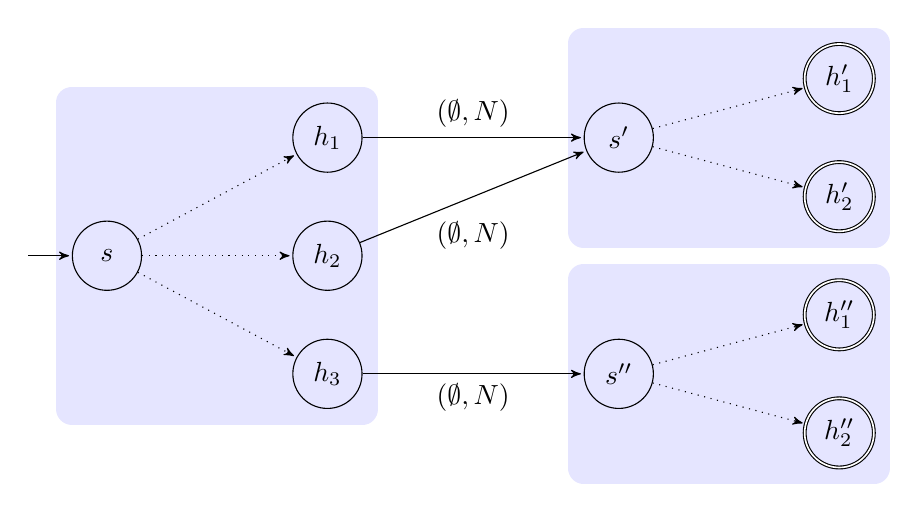
\begin{tikzpicture}[->,>=stealth',shorten >=1pt,auto,node distance=2.8cm]
  \begin{scope}
	  % Machine M
	  \node[state]          (M init)                                    {$s$};
	  \node[state]          (M exit 1)  [right of=M init,yshift= 1.5cm] {$h_1$};
	  \node[state]          (M exit 2)  [right of=M init,yshift= 0.0cm] {$h_2$};
	  \node[state]          (M exit 3)  [right of=M init,yshift=-1.5cm] {$h_3$};
	  \path (M init)
	  edge[dotted] (M exit 1)
	  edge[dotted] (M exit 2)
	  edge[dotted] (M exit 3);
	  \path (M init) ++(-1.0,0) edge (M init);
  \end{scope}
  \begin{scope}[xshift=6.5cm]
	  % Match-Machines
	  \begin{scope}[yshift=1.5cm]
		  % Accepting match machine
		  \node[state]          (M 1 init)                                        {$s'$};
		  \node[state, double]  (M 1 exit 1)  [right of=M 1 init, yshift= 0.75cm] {$h'_1$};
		  \node[state, double]  (M 1 exit 2)  [right of=M 1 init, yshift=-0.75cm] {$h'_2$};
		  \path (M 1 init)
		  edge[dotted] (M 1 exit 1)
		  edge[dotted] (M 1 exit 2);
	  \end{scope}
	  \begin{scope}[yshift=-1.5cm]
		  % Accepting match machine
		  \node[state]          (M 2 init)                                        {$s''$};
		  \node[state, double]  (M 2 exit 1)  [right of=M 2 init, yshift= 0.75cm] {$h''_1$};
		  \node[state, double]  (M 2 exit 2)  [right of=M 2 init, yshift=-0.75cm] {$h''_2$};
		  \path (M 2 init)
		  edge[dotted] (M 2 exit 1)
		  edge[dotted] (M 2 exit 2);
	  \end{scope}
  \end{scope}
  % Connecting edges
  \path
  (M exit 1) edge node[anchor=south] {$(\None, N)$} (M 1 init)
  (M exit 2) edge node[anchor=north,yshift=-0.2cm] {$(\None, N)$} (M 1 init)
  (M exit 3) edge node[anchor=north] {$(\None, N)$} (M 2 init);

  \begin{pgfonlayer}{background}
	  \filldraw [line width=4mm,join=round,blue!10]
	  (M   exit 1.north -| M   init.west) rectangle (M   exit 3.south -| M   exit 3.east)
	  (M 1 exit 1.north -| M 1 init.west) rectangle (M 1 exit 2.south -| M 1 exit 2.east)
	  (M 2 exit 1.north -| M 2 init.west) rectangle (M 2 exit 2.south -| M 2 exit 2.east);
  \end{pgfonlayer}
\end{tikzpicture}

  \caption{Example for a $\MS{match}$.  The left blue box stands for the first machine.  After it reaches on of the terminal states
    $s_1, \cdots, s_3$, it continues its execution either in the right top machine or in the right bottom case machine.
  The halting states of the match machine are exactly the halting states of the case-machines.}
  \label{fig:match-example}
\end{figure}

The idea of the \emph{match} operator is to first execute a machine and --- depending of the outcome of the execution --- continue the execution with
another machine.  To define this operator, the parametrised relational approach is in particular useful here.  This idea is illustrated in Figure
\ref{fig:match-example}.

First we fix an $n$-tape machine $M$ with a partition function $p$ into a finite type $F$.
We furthermore fix an $F$-indexed sequence of $n$-tape machines $M'_y$ (where $y:F$) with partitions $p'_y$ into another finite type $F'$.

The states of the machine are either states of $M$ or states of a machine $M'_y$.

$$Q_{\MS{match}} := Q_M + \depPair{y:F}{Q_{ \left( M'_{y} \right) }}$$

The initial state is $s_{\MS{match}} := s_M$.  Now we define the new $\gamma_{\MS{match}}$.
\begin{alignat*}{2}
  \gamma_{\MS{match}} & (\inl q, \MS{symbols}) &&:=
  \begin{cases}
    \gamma_{M}(q, \MS{symbols})                                & h_M(q) = \false \\
    \left( s_{\left(M'_{p(q)}\right)}, (\None, N)^n \right)  & h_M(q) = \true
  \end{cases} \\
  \gamma_{\MS{match}} & (\inr (y, q), \MS{symbols}) &&:= \gamma_{\left({M'_y}\right)}(q, \MS{symbols})
\end{alignat*}
Informally:  If the machine is in a non-halting state of $M$, then it mimics the step of $M$.  If $\MS{match}$ is at a halting state $q$ of $M$, it
inserts a operation that just goes to the start state of the corresponding machine $M'_{p(q)}$.  If the machine is in a state from $M'_y$ then it
mimics the step from $M_y$.

The halting states are exactly the halting states of each $M_f$:
\begin{alignat*}{3}
  h_{\MS{match}} &~ (\inl      q) &&:= \false \\
  h_{\MS{match}} &~ (\inr (y, q)) &&:= h_{\left( M'_y \right)}(q)
\end{alignat*}

Now we want to specify the semantics of the match machine and give a quick overview about the verification.

First we have to specify the partition function $p_{match} \from Q_{match} \to F'$:
\begin{alignat*}{3}
  p_{\MS{match}} &~ (\inl      q) &&:= p'_{\left({p~q}\right)} \left( s_{ \left( M'_{ \left( p~q \right) } \right) } \right) \\
  p_{\MS{match}} &~ (\inr (y, q)) &&:= p'_y(q)
\end{alignat*}
Note that the machine can not halt in an inner state of $M$, thus the first case of the definition of $p_{match}$ is over-specified.

We have now defined all components of $\MS{match}$.

Now we proof the correctness of this operator.  We prove weak correctness and termination separately.
We generalised the idea of the correctness proofs from the sequence operator from Asperti et al.
However, they could not define the $\MS{match}$ machine, because they do not use parametrised relations.

To proof the correctness of this operator, we first show four more facts about the abstract $\MS{loop}$ function.

\subsubsection{Weak correctness of $\MS{merge}$}

Let $R:\Rel~{\Tapes{n}}~(F \times \Tapes{n})$ be a parametrised relation for $M$ and $R'_y:\Rel~\Tapes{n}~(F' \times \Tapes{n})$ be a family
of relations for each case-machine $M'_y$.

We can show that if $M$ realises $R$ and each $M'_y$ realises $R'_y$ weakly, then $\MS{match}$ realises
$$R_\MS{match} := \bigcup_{y:F} (R \at y) \circ R'_y.$$
Note that this relation is a quite intuitive and a precise description of the behaviour of our defined operator:  First a copy of $M$ runs and may
terminates into a state that corresponds to some $y$ and then we run a copy of the machine $M_y$.

To do this, we have to show that if $\MS{match}$ terminates into a state $c$, then $M$ terminates to some state $c_1$ and the corresponding machine
$M'_y$ (where $y := p~\left( \MS{cstate}(c_1) \right)$), called \emph{continuation machine} of $c_1$, executes to a state $c_2$ that corresponds to
$c$.

We use two lemmas from Asperti et al.  The first tells us, informally, if $M'$ simulates $M$ and $M'$ terminates, then $M$ terminates in the
corresponding state.

\begin{lemma}[Unlift $\MS{loop}$]
  \label{lem:loop-unlift}
  Let $A$ be the abstract type for the simulated machine, $B$ the abstract type for the simulator machine.
  We need step functions $f \from A \to A$, $g \from B \to B$ and halting functions $h \from A \to \Bool$, $h' \from B \to \Bool$.

  Furthermore, let $\MS{unlift} \from B \to \Option A$ be a function that translates states simulated states to its original states, such that
  $(\forall a: A,~b: B,~\MS{unlift}~b = \Some a \rightarrow p~a = \false \rightarrow \MS{unlift}~(f'~b) = \Some{f a})$
  and
  $\forall a: A,~b: B,~\MS{unlift}~b = \Some a \rightarrow p~a = p'~b$.

  Let then $a:A$ and $b:B$, such that $\MS{unlift}~b = \Some{a}$.

  Let $x':B$ and $k:\Nat$, such that $\MS{loop}~k~f'~p'~b = \Some{x'}$.

  Then there exists an $x:A$, such that $\MS{loop}~k~f~p~a = \Some x = \MS{unlift}~x'$.
\end{lemma}
\begin{proof}
  This can be shown per induction on $k:\Nat$.
\end{proof}

The second fact says informally, that if an execution consists of two parts, these execution can be separated.

\begin{lemma}[Split $\MS{loop}$]
  \label{lem:loop-split}
  Let $A$ be a type, $f \from A \to A$ a step function, $p, q \from A \to \Bool$ halting functions, and $a_1, a_3:A$.

  Suppose that $\forall a:A,~p~a = \false \rightarrow q~b = \false$ and $\MS{loop}~k~f~q~a_1 = \Some{a_3}$.

  Then there exists a step counts $k_1, k_2$ and an intermediate value $a_2:A$, such that
  $\MS{loop}~k_1~f~p~a_1 = \Some{a_2}$ and $\MS{loop}~k_2~f~q~a_2 = \Some{a_3}$, and $k = k_1 + k_2$.
\end{lemma}

With the help of Lemma \ref{lem:loop-unlift} and \ref{lem:loop-split}, we want to show the following Lemma.
\begin{lemma}[Split $\MS{match}$]
  \label{lem:match-split}
  Let $k:\Nat$, $t:\Tapes{n}$, and $res:\MS{Conf}(\MS{match})$.
  If $\MS{exec}~\MS{match} t = \Some{res}$ then
  there exists $k_1,k_2:\Nat$, a configuration $c_1$ of $M$ and a configuration $c_2s$ of the successor-machine of $c_1$,
  such that $M$ terminates (with $t$ as initial tapes) in $k$ steps into $\Some{c_1}$ and the successor-machine of $c_1$ terminates (with the tapes of
  $c_1$ as initial tapes) into $\Some{c_2}$ and $res$ corresponds to $c_2$.
\end{lemma}
\begin{proof}
  We use \ref{lem:loop-unlift} twice and \ref{lem:loop-split} once.  Therefore, we need an $\MS{unlift}$ function for states of $M$ and a family of
  $\MS{unflift}$ functions for states from the machines $M_y$.  The proof is very technical and we omit it here.
\end{proof}

\begin{lemma}[Correctness of $\MS{match}$]
  \label{lem:match}
  If $M \VDash_p R$ and for each $y:F$, $M'_y \VDash_{p'_y} R'_y$, then
  $$\MS{match} \VDash \bigcup_{y:F} (R \at y) \circ R'_y$$
\end{lemma}

\subsubsection{Termination of $\MS{match}$}

The idea for termination is, that when $M$ terminates into a state $c_1$ the successor Machine $M_y$ terminates into $c_2$, then $\MS{match}$
terminates into the lifted state of $c_2$.

We show again two lemmas introduced by Asperti et al.
The first fact make it precise what it means that $M'$ ``runs a copy of $M$''.


\begin{figure}
  \center
  \begin{tikzcd}
    \Some{c'_2} & \Some{c_2} \arrow[l, "\MS{lift}" above, red] \\
    c' \arrow[u, "\MS{loop}~g~k", rightsquigarrow] & c \arrow[u, "\MS{loop}~f~k", rightsquigarrow, swap] \arrow[l, "\MS{lift}"] \\
    c'_1 \arrow[u, "g"] & c_1 \arrow[u, "f"] \arrow[l, "\MS{lift}"]
  \end{tikzcd}
  \caption{The step-case of the proof of Lemma \ref{lem:loop-lift} where we assume $h(c_1) = \false$ and conclude $h'(\MS{lift}(c_1)) = \false$.
  The inductive hypothesis gives us the red line.}
  \label{fig:proof-loop-lift}
\end{figure}
\begin{lemma}[Lift $\MS{loop}$]
  \label{lem:loop-lift}
  Let $A$ be the abstract type for the simulated machine, $B$ the abstract type for the simulator machine.
  We need step functions $f \from A \to A$, $g \from B \to B$ and halting functions $h \from A \to \Bool$, $h' \from B \to \Bool$.

  Furthermore, let $\MS{lift} \from A \to B$ be a function that lifts state from $A$ to $B$ that is in every state compatible with the step function and
  in halting states of $A$ compatible with the halting functions, i.e.
  $\forall x:A,~h'~(\MS{lift}~x) = h~x$ and $\forall x:A,~h~x = \false \rightarrow \MS{lift}~(f~x) = g~(\MS{lift}~x)$.

  Let $k:\Nat$ be a number of steps, and $c_1, c_2:A$ be abstract configurations.
  If $\MS{loop}~k~f~h~c_1 = \Some{c_2}$, then $\MS{loop}~k~g~h'~(\MS{lift}~c_1) = \Some{\MS{lift}~c_2}$.
\end{lemma}
\begin{proof}
  This can be proven by induction on $k:\Nat$.  The cases where $k=0$ or $h(c_1) = \true$ are trivial.
  The remaining case is depicted in Figure \ref{fig:proof-loop-lift} as a commuting diagram.
\end{proof}

The next fact makes it precise what it means that ``an execution gets continued''.

\begin{lemma}[Merge loop]
  \label{lem:loop-merge}
  Let $A$ be the abstract state type and $h, h' \from A \to \Bool$ two halting functions.
  Let $h$ and $h'$ correspond in non-halting states of $h$, i.e.  $\forall a:A,~h~a = \false \rightarrow h'~a = \false$.
  Let $k_1, k_2:\Nat$ be step counts, and $a_1, a_2, a_3:A$ be configurations, such that
  $\MS{loop}~k_1~f~h~a_1 = \Some{a_2}$, and $\MS{loop}~k_2~f~h'~a_2 = \Some{a_3}$.
  Then $\MS{loop}~(k_1 + k_2)~f~h'~a_1 = \Some{a_3}$.
\end{lemma}
\begin{proof}
  By induction on $k_1:\Nat$ with Lemma \ref{lem:loop}.
\end{proof}

% TODO: lift explizit angeben
\begin{lemma}[Total $\MS{match}$]
  \label{lem:match-merge}
  Let $t:\Tapes{n}$ and $k_1, k_2:\Nat$.
  Let $c_1$ be a configuration of $M$ and $c_2$ be a configuration of the successor machine of $c_1$.
  If $\MS{exec}~M~t~k_1 = \Some{c_1}$ and $\MS{exec}~M_y~(\MS{ctapes}~c_1)~k_2 = \Some{c_2}$ (where $M_y$ is the successor machine of $c_1$), then
  $\MS{exec}~\MS{match}~t~(1+k_1+k_2)$ is the configuration of $\MS{match}$ that corresponds to $c_2$.
\end{lemma}
\begin{proof}
  Consequence of Lemmas \ref{lem:loop-lift} and \ref{lem:loop-merge}.  We omit the proof here since it is very technical.
\end{proof}

An immediate consequence is the strong correctness of $\MS{loop}$.

\begin{lemma}[Strong correctness of $\MS{match}$]
  \label{lem:match-realise}
  If $M \vDash_p R$ (or $\vDash_p^{k_1}$ for some $k_1:\Nat$) and for each $y:F$, $M_y \vDash_{p'_y} R'_y$ (or $\vDash_{p'_y}^{k_2}$ for some
  $k_2:\Nat$), then
  $$\MS{match} \vDash \bigcup_{y:F} (R \at y) \circ R'_y$$
  (or $\vDash^{1+k_1+k_2}$).
\end{lemma}
\begin{proof}
  Both claims (strong realisation and realisation in constant time) are immediate consequences of Lemma \ref{lem:match-merge}.
\end{proof}

The claim for the relation $\downarrow$ is a bit more complicated to express.

\begin{lemma}[Termination of $\MS{match}$]
  \label{lem:match-terminates}
  Let $T$ be a termination relation for $M$ and $T'_y$ a family of termination relation for each machine $M'_y$.
  Let furthermore $R$ be a correctness relation for $M$ and $R$ be functional on $T$.
  Let $M \downarrow T$ and $M'_y \downarrow T'_y$ for each $y:F$.
  Then
  \begin{multline*}
    \MS{match} \downarrow
    \bigcup_{y:F}
    \setMap{(t:\Tapes{n}, k_3 :\Nat)}{\exists~k_1,k_2:\Nat,~\exists~t':\Tapes{n},~ \\
    R~t~(y, t') \land T~t~k_1 \land T'_y~t'~k_2 \land k_1+k_2 < k_3}.
  \end{multline*}
\end{lemma}
\begin{proof}
  The claim is an immediate consequences of Lemma \ref{lem:match-merge}, also using \ref{lem:loop}.
\end{proof}

It seems strange that we need a correctness relation in this Lemma.  The reason is that we need to know the corresponding value of $F$, where $M$
terminated, and this information is not encoded inside $\downarrow$.  However, to show the weak realisation of $\MS{match}$ we need to show the weak
$M \vDash R$.  Therefore we could just use this $R$ and show that $R$ is functional on $T$.  $R$ and $T$ should always be defined in such way.
Another possibility is to use the canonical relation.  We already know that it is functional, see Lemma \ref{lem:canonical-relation}.

\subsubsection{Derivated operators}

Now that we have a match combinator, sequential composition and boolean if can be reduced to it, by arguing that sequential composition is just a
trivial matching from any states of $M_1$ to $M_2$, and a boolean if amounts to matching over a boolean value:


\begin{definition}[Sequential composition]
  \label{def:seq}
  Let $M_1, M_2$ be an $n$-tape machines over $\Sigma$ with the partitioning function $p_1 \from Q_1 \to F_1$ and $p_2 \from Q_2 \to F_2$,
  respectively.  Then we define the \emph{sequential composition} of $M_1$ and $M_2$:
  $$M_1 \mseq M_2 := \mmatch~(M_1, p_1)~(\lam y (M_2, p_2))$$
\end{definition}

\begin{corollary}[Correctness of sequential composition]
  \label{lem:seq}
  If $M_1 \vDash R_1$ and $M_2 \vDash R_2$, then $M_1 \mseq M_2 \vDash R_1 \circ \hideParam R_2$.
\end{corollary}

\begin{definition}[Boolean if]
  \label{def:if}
  Let $M_1, M_2, M_3$ be an $n$-tape Turing machines over $\Sigma$.
  Let $p_1 \from Q_1 \to \Bool$ and $p_2 \from Q_2 \to F', p_3 \from Q_3 \to F'$ be partitioning functions.
  Then we define \emph{boolean if}:
  $$\mif{M_1}{M_2}{M_3} := \MS{match}~(M_1, p_1) \left(\lam b \begin{cases} (M_2; p_2) & b = \true \\ (M_3; p_3) & b = \false \end{cases} \right)$$
\end{definition}

\begin{corollary}[Correctness of boolean if]
  \label{lem:if}
  If $M_1 \vDash R_1$ and $M_2 \vDash R_2$ and $M_3 \vDash R_3$, then
  $\mif{M_1}{M_2}{M_3} \vDash (R_1 \at \true) \circ R_2 \cup (R_1 \at \false) \circ R_3$.
\end{corollary}


\subsection{While}

\begin{figure}
  \center
  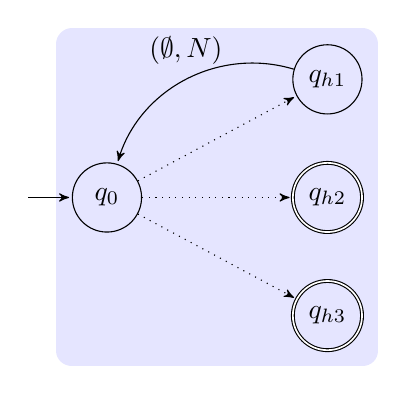
\begin{tikzpicture}[->,>=stealth',shorten >=1pt,auto,node distance=2.8cm,bend angle=45]
    \begin{scope}
      % Machine M
      \node[state]          (M init)                                    {$q_0$};
      \node[state]          (M exit 1)  [right of=M init,yshift= 1.5cm] {$q_{h1}$};
      \node[state, double]  (M exit 2)  [right of=M init,yshift= 0.0cm] {$q_{h2}$};
      \node[state, double]  (M exit 3)  [right of=M init,yshift=-1.5cm] {$q_{h3}$};
      \path (M init)
      edge[dotted]          (M exit 1)
      edge[dotted]  (M exit 2)
      edge[dotted]  (M exit 3);
      \path (M init) ++(-1.0,0) edge (M init);
      \path (M exit 1) edge[bend right] node[anchor=south,yshift=0.2em] {$(\None, N)$} (M init);
    \end{scope}

    \begin{pgfonlayer}{background}
      \filldraw [line width=4mm,join=round,blue!10]
      (M   exit 1.north -| M   init.west) rectangle (M   exit 3.south -| M   exit 3.east);
    \end{pgfonlayer}
  \end{tikzpicture}
  \caption{Example for a do-while-loop.  When the machine reaches the state $q_{h1}$ it restarts.  It holds in the final states $q_{h2}$ and $q_{h3}$.}
  \label{fig:while-example}
\end{figure}

The $\MS{while}$ operator implements a \emph{do-while-loop}.  The loop condition, however, is encoded through the boolean partition
function of the terminal states:  We insert transitions from the ``positive'' halting states.  This idea is depicted in Figure
\ref{fig:while-example}.  We generalise the proofs and definitions from Asperti et al.

We define the while-machine formally.  Let $M$ be a machine with a boolean partition function $p \from Q_M \to \Bool \times F$, where $F$ is an
arbitrary finite type.  Then the transition function of $\MS{while}$ is
$$\gamma_{\MS{while}} (q, \MS{symbols}) :=
  \begin{cases}
    \bigl( q_0, (\None, N)^n \bigr) & h_M(q) = \true \land \#1(p~q) = \true \\
    \gamma_M(q, \MS{symbols})           & \txt{else}
  \end{cases} $$
The halting states are the ``negative'' halting states of $M$:
$$h_{\MS{while}}(q) = \true \iff h_M(q) = \true \land \#1(p~q) = \false.$$

The partition function of $\MS{while}$ just returns the additional parameter of $p$:
$$p_{\MS{while}}(q) := \#2(p~q).$$

We now defined every component of $\MS{while}$.

The semantics of $\MS{while}$ can be defined with help of the Kleene star:

\begin{lemma}[weak correctness of $\MS{while}$]
  \label{lem:while-wrealise}
  If $M \VDash R$, then
  $$ \MS{while} \VDash
  \left( \bigcup_{y:F} R\at{(\true, y)} \right)^* \circ
  \setMap{(t, (y, t'))}{R~t~((\false, y), t')}
  $$
\end{lemma}

The correctness proof is similar to the correctness proof of the $\mmatch$ machine.  We do an additional complete induction over the number of steps.

However, we can not replace $\VDash$ with $\vDash$ in Lemma \ref{lem:while-wrealise}, because we do not know weather the loop will terminate.
We need an additional lemma to prove that a $\MS{while}$ machine terminates.

\begin{lemma}[Termination of $\MS{while}$]
  \label{lem:while-term}
  Let $M \VDash R$ and $M \downarrow T$.  We define $T_{\MS{while}}$ inductively:

  $$ \inferrule{R~t_1~((\false, y), t_2) \and T~t_1~k_1 \and k_1 \le k_2}{T_{\MS{while}}~t_1~k_2} $$
  $$ \inferrule{R~t_1~((\true,  y), t_2) \and T_{\MS{while}}~t_2~k_2 \and k_1 + k_2 < k_3}{T_{\MS{while}}~t_1~k_3} $$

  Let $R$ be functional on $T$.  Then
  \begin{enumerate}
    \item $R$ is functional on $T_{\MS{while}}$.
    \item $\MS{while} \downarrow T_{\MS{while}}$.
  \end{enumerate}
\end{lemma}
\begin{proof}
  Claim 1 follows by induction on $T_{\MS{while}}$.
  Claim 2 follows by complete induction on the number of steps and case distinction on $T_{\MS{while}}$ with a similarly approach as the termination
  proof of $\MS{match}$.
\end{proof}

\section{Machine transformations}
\label{sec:transformations}

Using the operators above, we can build and verify small machines with ease.  However, to compose machines, they have to agree in their alphabet and in
their number of tapes.  Because this is not always the case, we introduce new operators, that ``enlarge'' a given machine by either introducing new
tapes or by ``translating'' alphabets.


\subsection{\texorpdfstring{$m,n$}{m,n}-lift}
\label{sub:m-n}

\begin{figure}
  \center
  \begin{tikzpicture}
    \begin{scope}
      \node(a0)[yshift=-0 cm]  {$0$};
      \node(a1)[yshift=-1 cm]  {$1$};
      \node(a2)[yshift=-2 cm]  {$2$};
    \end{scope}
    \begin{scope}[xshift=4cm, yshift=0cm]
      \node(b0)[yshift=-0 cm] {$0$};
      \node(b1)[yshift=-1 cm] {$1$};
      \node(b2)[yshift=-2 cm] {$2$};
      \node(b3)[yshift=-3 cm] {$3$};
      \node(b4)[yshift=-4 cm] {$4$};
    \end{scope}
    \begin{scope}[xshift=5cm, yshift=-3cm]
      \node(none)             {$\None$};
    \end{scope}
    \path (a0) edge[<->] (b1);
    \path (a1) edge[<->] (b0);
    \path (a2) edge[<->] (b3);
    \path (b2) edge[-> ] (none);
    \path (b4) edge[-> ] (none);
  \end{tikzpicture}
  \caption{An example for a retract between tape indexes, for $m=3$ and $n=5$.  The arrows from the left to the right correspond to the
    function $f$. The function $g$ maps $0$ back to $\Some{1}$, $1$ to $\Some{0}$ and $3$ to $\Some{2}$; all other values are mapped to $\None$.
  This retract is encoded as the vector $[1,0,3]$.}
  \label{fig:m-n-lift-example-mapping}
\end{figure}

The most of our machines do really only work on one or two tapes, but they have to be embedded into machines with more tapes.  There are two possible
routes to follow: One way to solve this problem could be to define all these machines as $n$-tape machines and give them the tape-indexes on which the
machine should operate.  We could also define those machines as e.g. two-tapes machines and then define an ``lift'' operation that can automatically
build an arbitrary big machine that only operates on two of its tapes and emulates the behaviour of the smaller machine.

However, the first approach seems unsatisfying, because definition and verification of small Turing machines is easier.  We don't want to struggle
every time with this, when we define a new machine.

Therefore we introduce the $m,n$-lift. For $n \ge m$, given a $m$-tape Turing machine it yields an $n$-tape Turing machine that has exactly the
same behaviour but ignores $n-m$ of the tapes.  The operator takes a retract from $m$-tape indexes to $n$-tape indexes.  It has to be a retract and
hence, because the behaviour of a tape can not be ``duplicated'', because tapes can behave different in different contexts.  We need the inversion
function of the retract to translate the indexes back in the transition function $\gamma$.

To encode this retract from $\Fin_m$ to $\Fin_n$, we use \emph{index vectors} of type $\Fin_n^m$, that must be duplicate free.  This encoding of the retract makes the implementation more convenient.

For example, with $m=3$ and $n=5$ and we can  map the tape $0$ to the tape $1$, tape $1$ to tape $0$, and tape $2$ to tape $3$, as depicted in Figure
\ref{fig:m-n-lift-example-mapping}.

For the definition and verification of the $m,n$-lift we need two functions.
First we need the dependent function
$\MS{inject} \from \forall m, n:\Nat,~\Fin_n^m \to X^n \to X^m \to X^n$,
that inserts all values in the image of $f$ from $m$-vector into the $n$-vector.  We define it per dependent recursion over the size $m$:
\begin{alignat*}{6}
  \MS{inject}&&~ 0         && ~ n &&~ \nil                &&~ \MS{def} &&~ \nil      &:= \MS{def} \\
  \MS{inject}&&~ (\MS S~m) && ~ n &&~ [i :: \MS{index'}]  &&~ \MS{def} &&~ (v :: V') &:= \MS{replace}~(\MS{inject}~m~n~\MS{index'} V')~i~v
\end{alignat*}

Let $M$ be a $m$-tape Turing machine over $\Sigma$.  Let $n \ge m$ and let $\MS{indexes}:\Fin_n^m$ be an index vector.
(We will from now on call the function $\MS{inject}$ implicitly with $\MS{indexes}$.)

The second function we need is $\MS{reorder} \from X^n \to X^m$, that selects the values of the indexes in the image of $f$:
$$\MS{reorder}~Z := \map~(\MS{nth}~Z)~\MS{indexes}.$$

Using these two functions we can define the transition function $\gamma_{\MS{lift}}$:
\begin{alignat*}{3}
  &\gamma_{\MS{lift}} (q, \MS{sym})  &~:=~& \mlet {(q', \MS{act}) := \gamma_M(q, \MS{reorder}~\MS{sym})}{\\
  &                                  &~  ~& (q',\MS{inject}~\MS{act}~(\None, N)^n)}
\end{alignat*}

The states, initial state, final states, the alphabet, and the state partitioning of the lift-machine are inherited from $M$.
Thus, we have defined all components of the lift machine; from other chapters we will refer to it with $\MS{lift}~\MS{indexes}~M$.

\begin{definition}[Relational $m,n$-lift]
  \label{def:m,n-rellift}
  For $R : \Rel~\Tapes{n}~(F \times \Tapes{n})$:
  \begin{multline*}
    R_{\MS{lift}}(R) := \setMap{(\MS{input}, (y, \MS{output}))}{R~(\MS{reorder}~\MS{input})~(y,\MS{reorder}~\MS{output})} \cap \\
    \ignoreParam \setMap{(\MS{input},\MS{output})}{\forall j:\Fin_n, j \notin \MS{indexes} \rightarrow \MS{input}[j] = \MS{output}[j]}
  \end{multline*}
  For $T : \Rel~\Tapes{n}~\Nat$: $ T_{\MS{lift}}(T) := \setMap{(\MS{input}, k)}{T~(\MS{reorder}~\MS{input})~k} $.
\end{definition}

\begin{lemma}[Correctness of the $m,n$-lift]
  \label{lem:m,n-correctness}
  For correctness relations $R$ and termination relations $T$:
  \begin{enumerate}
    \item
      If $M \VDash R$, then $\MS{lift} \VDash R_{\MS{lift}}(R)$.
    \item
      If $M \downarrow T$, then $\MS{lift} \downarrow T_{\MS{lift}}(T)$.
  \end{enumerate}
\end{lemma}

\subsection{\texorpdfstring{$\Sigma,\Tau$}{Sigma,Gamma}-Lift}
\label{sub:sigma-gamma}

\begin{figure}
  \center
  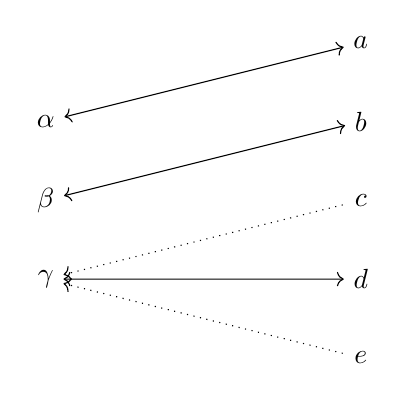
\begin{tikzpicture}
    \begin{scope}
      % Symbols of $\Sigma$
      % FIXME This loop does not work!
      % \foreach \x / \y in {0 / \alpha, 1 / \beta, 2 / \gamma}
      %   \node(sigma\x)[yshift=-\x cm] {$\y$};;
      \node(alpha)[yshift=-0 cm] {$\alpha$};
      \node(beta) [yshift=-1 cm] {$\beta$};
      \node(gamma)[yshift=-2 cm] {$\gamma$};
    \end{scope}
    \begin{scope}[xshift=4cm, yshift=1cm]
      % Symbols of $\Tau$
      \node(a)[yshift=-0 cm] {$a$};
      \node(b)[yshift=-1 cm] {$b$};
      \node(c)[yshift=-2 cm] {$c$};
      \node(d)[yshift=-3 cm] {$d$};
      \node(e)[yshift=-4 cm] {$e$};
    \end{scope}
    \path (alpha) edge[<->] (a);
    \path (beta)  edge[<->] (b);
    \path (gamma) edge[<->] (d);
    \path (gamma) edge[<-, dotted] (c);
    \path (gamma) edge[<-, dotted] (e);
  \end{tikzpicture}
  \caption{An example for a retract plus default element between the alphabets $\Sigma = \setOf{\alpha, \beta, \gamma}$ and $\Tau =
    \setOf{a,b,c,d,e}$.  The symbols $c$ and $e$ are not in the image of $f$ and are implicitly mapped to $\gamma$, the chosen default element in
  $\Sigma$.}
\label{fig:sigma-tau-lift-example-mapping}
\end{figure}

Similarly to the $m,n$-Lift, the $\Sigma,\Tau$-Lift extends the alphabet of a Turing machine.  The operator gets a retract $(f,g) \from \Sigma
\hookrightarrow \Tau$.  However we also have to give an symbol $\MS{default}:\Sigma$, for the symbols in $\Tau$ that can not be mapped back to
$\Sigma$.  This idea is illustrated in Figure \ref{fig:sigma-tau-lift-example-mapping}.

Let $M$ be an $n$-tape Turing machine over $\Sigma$.  The alphabet of the lift-machine is $\Tau$.  The states, initial states, the final states, and
the partitioning are inherited from $M$.  To define the transition function of the list, we have to define some functions again.

There is a dependent function $\map_\Tape:\forall X, Y:\MS{finType},~(X \to Y) \to \Tape(X) \to \Tape(Y)$, that applies a function to a each symbol
on of a tape and preserves the position of the pointer.
For convenience, we also introduce the functions $\map_\Option$, $\map_\MS{left}$, $\map_\MS{right}$, and $\map_\MS{Act}$:
\begin{alignat*}{4}
  \map_\Option &&~ f && a &:=
    \begin{cases}
      \Some{f~a'} & a = \Some{a'} \\
      \None       & a = \None
    \end{cases} \\
    \map_\MS{left}  &&~ f &&~ (a, b) &:= (f~a, b) \\
    \map_\MS{right} &&~ f &&~ (a, b) &:= (a, f~b) \\
    \map_\MS{Act}   &&~ f &&         &:= \map_\MS{left}~(\map_\Option~f)
\end{alignat*}
% XXX Define Act
Note that $map_\MS{Act}$ applies a function to the optional symbol of an action tuple.

Then we can define the function $g' \from \Tau \to \Sigma$, that is $g$ extended by $\MS{default}$:
\begin{align*}
  \MS{surject}~\tau :=
  \begin{cases}
    s            & g~\tau = \Some{s} \\
    \MS{default} & g~\tau = \None
  \end{cases}
\end{align*}

Furthermore we define $\MS{surject\_tape}(tape) := \map_\Tape~\MS{surject}~t$ and
$\MS{surject\_tapes}(\MS{tapes}) := \map~\MS{surject\_tape}~\MS{tapes}$.
Now we can finally define the transition function $\gamma_\MS{lift}$ of the $\Sigma,\Tau$-lift:
\begin{alignat*}{3}
  &\gamma_\MS{lift} (q, sym) &~:=~& \mlet {(q', acts) := \gamma_M(q, \map~(\map_\Option~\MS{surject})~sym)}{\\
  &                          &~  ~& (q', \map~(\map_\MS{Act} f)~acts)}
\end{alignat*}

Now, that we have defined all components the $\Sigma,\Tau$-lift, from other chapters we will refer to it with $\MS{lift}~(f,g)~M$.

\begin{definition}[Relational $\Sigma,\Tau$-lift]
  \label{def:sigma,tau-rellift}
  For $R : \Rel~\Tapes{n}~(F \times \Tapes{n})$:
  $$R_\MS{lift}(R) := \setMap{\MS{input} (y, \MS{output})}{R~(\MS{surject\_tapes}~\MS{input})~(y, \MS{surject\_tapes~\MS{output}})}$$
  For $T : \Rel~\Tapes{n}~\Nat$:
  $T_\MS{lift}(T) := \setMap{(\MS{input}, k)}{T (\MS{surject\_tapes}~\MS{input})~k}$
\end{definition}
\begin{lemma}[Correctness of the $\Sigma,\Tau$-lift]
  \label{lem:sigma-tau}
  For correctness relations $R$ and termination relations $T$:
  \begin{enumerate}
    \item
      If $M \VDash R$, then $\MS{lift} \VDash R_{\MS{lift}}(R)$.
    \item
      If $M \downarrow T$, then $\MS{lift} \downarrow T_{\MS{lift}}(T)$.
  \end{enumerate}
\end{lemma}


\subsection{Mirror machine}
\label{sub:mirror}

The two machine transformations we have seen, modify either the number of tapes or the content of the tapes, but don't modify actions.
This operator swaps all the directions:  If the original machine would move one pointer to the left, this machine would move that pointer to the right.

This is in particular useful, for example, if we define and certify a machine, that moves its pointer to the right.  Then we don't want to repeat all
definitions and proofs, just for a machine, that moves its pointer to the left.


To define the $\MS{mirror}$ machine, we need the involutive and bijective function $\MS{mirror\_mv} \from \Move \to \Move$ that swaps $L$ and $R$.
\begin{alignat*}{3}
  &\gamma_\MS{mirror}~\MS{\MS{qsym}} &~:=~& \mlet {(q, \MS{acts}) := \gamma_M (\MS{qsym})}{\\
  &                                  &~  ~& (q', \map~(\MS{\MS{map\_right}~\MS{mirror\_move}})~\MS{acts})}
\end{alignat*}
The number of taeps, states, the partitioning function, the halting states and the initial state are inherited from $M$.  We write $\MS{mirror}$.

We define a function that mirrors a tape, where the pointer stays at the same position:
\begin{alignat*}{3}
  \MS{mirror\_tape}&~\niltape            &&:= \niltape \\
  \MS{mirror\_tape}&~\leftof{r}{rs}      &&:= \rightof{\rev~rs}{r} \\
  \MS{mirror\_tape}&~\rightof{ls}{l}     &&:= \leftof{l}{\rev~ls} \\
  \MS{mirror\_tape}&~\midtape{ls}{m}{rs} &&:= \midtape{\rev~rs}{m}{\rev~ls} \\
  \MS{mirror\_tapes}&                    &&:= \map~\MS{mirror\_tape}
\end{alignat*}
Note that this definition differs slightly from the definition in Coq, since we store the left lists already in reversed order.

\begin{lemma}[Correctnes of $\MS{mirror\_tape}$]
  \label{lem:mirror}
  Let $t$ be a tapes over an alphabet.  Then
  \begin{enumerate}
    \item $\MS{left} (\MS{mirror\_tape}~t) = \MS{right}~t$ and $\MS{right}(\MS{mirror\_tape}~t) = \MS{left} ~t$.
    \item $\MS{current}(\MS{mirror\_tape}~t) = \MS{current}~t$
    \item $\MS{mirror\_tape}$  is involutive and injective.
    \item $\MS{mirror\_tapes}$ is involutive and injective.
  \end{enumerate}
\end{lemma}
\begin{proof}
  Claims 1--3 follow by case analysis over $t$.
  Claim 4 follows by claim 3.
\end{proof}

% TODO: Definition of the mirror machine!

We observe the following behaviour of the $\MS{mirror}$ machine:  If we first mirror the tapes, then run the mirrored machine, and mirror the tapes
again, the resulting tapes are exactly the tapes that result when we run the original machine on the origial input tapes.
We express that behaviour as relations.
\begin{definition}[Relational mirror]
  \label{def:mirror-rellift}
  For $R : \Rel~\Tapes{n}~(F \times \Tapes{n})$:
  $$R_\MS{mirror}(R) := \setMap{(\MS{input}, (y, \MS{output}))}{R~(\map~\MS{mirror\_tape}~\MS{input})~(y, \map~\MS{mirror\_tape}~\MS{output})}$$
  For $T : \Rel~\Tapes{n}~\Nat$:
  $T_\MS{mirror}(T) := \setMap{(\MS{input}, k)}{T (\map~\MS{mirror\_tape}~\MS{input})~k}$
\end{definition}
\begin{lemma}[Correctness of $\MS{mirror}$]
  \label{lem:mirror-tm}
  For correctness relations $R$ and termination relations $T$:
  \begin{enumerate}
    \item
      If $M \VDash R$, then $\MS{mirror} \VDash R_{\MS{mirror}}(R)$.
    \item
      If $M \downarrow T$, then $\MS{mirror} \downarrow T_{\MS{mirror}}(T)$.
  \end{enumerate}
\end{lemma}

\section{Basic machines}

% TODO Present basic machiens here:
% TODO - Write
% TODO - Move

We introduce some basic $1$-tape classes machines (together with their partition functions) here, that are very helpful when combining machines.
They all do at most one simple step, for example write a symbol, or move the pointer.

The simplest class of $1$-tape machines is $\MS{nop}~y$, that does nothing and terminates in its initial state.  However, the partition function
returns $y$ for this state.
Let $F$ be a finite type and $y : F$.
Then we define the $1$-tape $\MS{nop}$ machine with its portioning function:
\begin{alignat*}{3}
  Q_     \MS{nop} &~  &&:= \Unit \\
  s_     \MS{nop} &~  &&:= \unit \\
  h_     \MS{nop} &~\_&&:= \true \\
  \gamma_\MS{nop} &~\_&&:= (\unit, (\None, N)^1) \\
  p_     \MS{nop} &~q &&:= y
\end{alignat*}

There are many ways how to express the correctness statement of this machine, e.g.:
\begin{lemma}[Correctness of $\MS{nop}$]
  \label{lem:nop-tm}
  For every $y \in F$:
  $$\MS{nop}~y \vDash^0 \setMap{(t_{in}, (y_{out}, t_{out}))}{t_{in}[0] = t_{out}[0] \land y_{out} = y}.$$
\end{lemma}
Note that we could also build an $n$-tape $\MS{nop}$ operator by applying the $m,n$-lift to the empty machine with $0$ tapes.


We also present a class of $1$-tape-$1$-step machines $\MS{read}$, that read a symbol and terminate into a state, that corresponds to this symbol.
Let $\Sigma$ be an alphabet.  Then the portioning function has the type $p_\MS{read} \from Q_\MS{read} \to \Option~\Sigma $.
The initial state is $\inl \true$, the final states are all other states.  It terminates in $(\inl \false)$ if and only if there is no current symbol
on the tape.  Else it terminates in the corresponding right state of the read symbol.
\begin{alignat*}{3}
  Q_     \MS{read} &~  &&:= \Bool + \Sigma \\
  s_     \MS{read} &~  &&:= \inl \true \\
  h_     \MS{read} &~q &&:= q \neq \inl \true \\
  \gamma_\MS{read} &~(\_, \MS{sym}) &&:=
  \begin{cases}
    (\inl \false, (\None, N)) & \MS{sym}[0] =\None \\
    (\inr a,      (\None, N)) & \MS{sym}[0] =\Some a
  \end{cases} \\
  p_     \MS{read} &~q &&:=
  \begin{cases}
    \Some a                   & q = \inl a \\
    \None                     & \txt{else}
  \end{cases}
\end{alignat*}

\begin{lemma}[Correctness of $\MS{read}$]
  \label{lem:read-tm}
  $\MS{read}$ realises the following relation in one step:
  $$\MS{read} \vDash^1 \setMap{(t_{in}, (y_{out}, t_{out}))}{t_{in}[0] = t_{out}[0] \land y_{out} = \MS{current}(t_{in}[0])}.$$
\end{lemma}

The next class of machines, $\MS{write}~x~y$, writes exactly on symbol $x:\Sigma$ to its tape and terminates in one step to a state corresponding $y$.
The definition is straight forward.
\begin{alignat*}{3}
  Q_     \MS{write} &~  &&:= \Bool \\
  s_     \MS{write} &~  &&:= \false \\
  h_     \MS{write} &~q &&:= q \\
  \gamma_\MS{write} &~\_&&:= (\true, (\Some x, N)^1) \\
  p_     \MS{write} &~\_&&:= y
\end{alignat*}
\begin{lemma}[Correctness of $\MS{write}$]
  \label{lem:write-tm}
  $$\MS{write} \vDash^1 \setMap{(t_{in}, (y_{out}, t_{out}))}{t_{out}[0] = \MS{wr}~(t_{in}[0])~\Some{x} \land y_{out} = y}.$$
\end{lemma}

The last operation-machine class we need is $\MS{move}~D~y$, where $D : \Move$ is an direction and $y : F$ is a parameter.
\begin{alignat*}{3}
  Q_     \MS{write} &~  &&:= \Bool \\
  s_     \MS{write} &~  &&:= \false \\
  h_     \MS{write} &~q &&:= q \\
  \gamma_\MS{write} &~\_&&:= (\true, (\None, D)^1) \\
  p_     \MS{write} &~\_&&:= y
\end{alignat*}
\begin{lemma}[Correctness of $\MS{move}$]
  \label{lem:move-tm}
  Let $D$ be a direction and $y : F$.  Then
  $$\MS{move} \vDash^1 \setMap{(t_{in}, (y_{out}, t_{out}))}{t_{out} = \MS{mv}_D (t_{in}[0]) \land y_{out} = y}.$$
\end{lemma}

We can use this operational machine, to build a machine that writes a certain string on a tape instead of only a single symbol.
Given a move direction $D : \Move$, a string $xs : \List~\Sigma$, and a parameter $y \in F$, we define this machine by recursion over the string,
using sequential composition:
\begin{alignat*}{3}
  \MS{write\_str}&~\nil         &&:= \MS{nop}~y \\
  \MS{write\_str}&~(x \cons xs) &&:= \MS{write}~x \mseq \MS{move}~D \mseq \MS{write\_str}~xs
\end{alignat*}

To define the correctness relation for this class of machines, we also use recursion on the string and define a function, that writes a string on a
tape:
\begin{alignat*}{3}
  \MS{write\_str'}~t &~\nil         &&:= t \\
  \MS{write\_str'}~t &~(x \cons xs) &&:= \MS{write\_str'}~(\MS{wr\_mv}~t~(\Some x, D))~xs
\end{alignat*}

\begin{lemma}[Correctness of $\MS{write\_string}$]
  \label{lem:write-string}
  For each string $xs : \List~\Sigma$ and direction $D : \Move$:
  $$\MS{write\_string}~D~xs \vDash^{4 \cdot \left|str\right|} \setMap{(t_{in}, (y_{out}, t_{out}))}{t_{out} = \MS{write\_str'}~t_{in}~xs \land
    y_{out} = y}.$$
\end{lemma}
\begin{proof}
  The idea is to recursively define a correctness relation $R~xs$ and show by induction on $xs$ that $\MS{write\_string}~xs$ realises $R~xs$ in
  $4 \cdot \left|str\right|$ steps using the correctness lemmas \ref{lem:seq}, \ref{lem:write-tm}, and \ref{lem:move-tm}.
  Then we show that $R~xs$ is a includes the correctness relation of $\MS{write\_string}$.
\end{proof}

\section{Encoding types}
\label{sec:encode}

The next step is to define what it means that a tape encodes a certain value.
Therefore we need a mechanism to linearise values to lists of symbols.
The key idea is the definition of \emph{encodable types}.

\begin{definition}[Codable type]
  \label{def:code}
  A type $X$ is \emph{encodable} over an alphabet $\Sigma$, if there exists an \emph{encoding function}
  $\MS{encode} \from X \to \List~\Sigma$, such that for all values $v_1, v_2:X$ and rest lists $r_1, r_2:\List~\Sigma$,
  if $\MS{encode}(x) \app r_1 = \MS{encode}(v_2) \app r_2$, then
  $v_1 = v_2$ and $r_1 = r_2$.

  If $X$ is encodable over $\Sigma$, then we will use the overloaded notation $\MS{encode}_{\Sigma}(x)$, to call the encoding function, or leave out
  $\Sigma$, if it is clear.  In the Coq implementation, this Definition is a type class.
\end{definition}

Note that this strong property implies injectivity of the encoding function.
It also implies that the encoding is a prefix encoding.

Our Coq development provides a library of encoding functions for typical types, for example:  $\Unit$, $\bot$, $\Option(X)$, $X+Y$, $X \times Y$,
$\List(X)$ and $\Nat$.  Note that each type can be encoded on different alphabets.  For example we can encode every finite type $F$ to the alphabet
$F$ itself.  But we could also encode finite types to $\Unit$.

\begin{example}[Encoding basic types]
  \label{ex:bacic-code}
  $\Unit$ and $\bot$ can be encoded over the empty alphabet, while every finite type $F$ can encode itself:
  \begin{alignat*}{3}
    \MS{encode}&_F    &&~(f:F)     &&:= [f] \\
    \MS{encode}&_\bot &&~(x:\bot)  &&:= [] \\
    \MS{encode}&_\Unit&&~(x:\Unit) &&:= [] \\
  \end{alignat*}
\end{example}

To encode more complex types we need a mechanism to extend an alphabet.
\begin{lemma}[Alphabet mapping]
  \label{lem:code-map}
  Let $X$ be a type and $\Sigma, \Tau$ be alphabets.
  Let $\MS{encode}_\Sigma \from X \to \List~\Sigma$ is an encoding function for $X$ on $\Sigma$ and
  let $(f,g) \from \Sigma \hookrightarrow \Tau$ be a retract.
  Then $\MS{encode}_\Tau \from X \to \List~\Tau := \map~f~(\MS{encode}~x)$ is an encoding function for $X$ on $\Tau$.
\end{lemma}

\begin{proof}
  To show that this is a valid encoding function, it suffices to show the following lemma:
  \begin{multline*}
    \forall v_1,v_2:X,~\forall r_1, r_2:\List(\Sigma),~\forall R_1, R_2:\List(\Tau),\\
    \map~f~(\MS{encode}~v_1 \app r_1) \app R_1 = \map~(\MS{encode}~v_2 \app r_2) \app R_2 \Rightarrow \\
    v_1 = v_1 \land \map~f~r_1 \app R_1 = \map~f~r_2 \app R_2.
  \end{multline*}
  This can be shown by double-induction over $R_1, R_2:\List~\Tau$, using some lemmas.
  In particular we have to create a tight retract $(f, g') \from \Sigma \hookrightarrow \Tau$.
  That is possible because alphabets are discrete.
\end{proof}


\begin{corollary}[Extend alphabets]
  \label{lem:extend-alphabet}
  Let $X, Y$ be types encodable over $\Sigma$ and $\Tau$, respectively.
  Using Lemma \ref{lem:code-map} we can build new encoding functions:
  \begin{alignat*}{3}
    \MS{encode}&_{\Sigma + \Tau}    &&\from X \to \List(\Sigma + \Tau) \\
    \MS{encode}&_{\Sigma + \Tau}    &&\from Y \to \List(\Sigma + \Tau) \\
    \MS{encode}&_{\Option(\Sigma)}  &&\from X \to \List(\Option(\Sigma))
  \end{alignat*}
  Furthermore, if $X$ is encodable over $\Sigma+\bot$, then $X$ is encodable over $\Sigma$.
  Also, if $X$ is encodable over $\Sigma+\Tau$, then $X$ is encodable over $\Tau+\Sigma$.
\end{corollary}

Using Corollary \ref{lem:extend-alphabet} we can construct more encoding functions for compound types:
\begin{corollary}[Encoding compound types]
  \label{lem:code-compound}
  Let $X, Y$ be types encodable over $\Sigma$ and $\Tau$, respectively.
  Then the following functions are encoding functions:
  \begin{alignat*}{3}
    \MS{encode}&_{\Sigma + \Tau + \Bool}&(\inl x) &:= \inr \false \cons \MS{encode}(x) \\
    \MS{encode}&_{\Sigma + \Tau + \Bool}&(\inl y) &:= \inr \true  \cons \MS{encode}(y) \\
    \MS{encode}&_{\Sigma + \Bool}& (\nil)         &:= \inr \false \\
    \MS{encode}&_{\Sigma + \Bool}& (x :: xs)      &:= \inr \true \cons \MS{encode}(x) \app \MS{encode}_{\Sigma + \Bool}(xs)
  \end{alignat*}
  Note that for each application of $\MS{encode}(x)$ and $\MS{encode}(y)$ we have to use $\map$.
  Also note that the list encoding is the only encoding that needs the strong encoding property.  All other encoding functions so far can be built
  with only the injectivity property.
\end{corollary}

We will now see how we can encode tuples.
Technically, to encode tuples of type $X \times Y$, where $X$ and $Y$ are both encodable over $\Sigma$, we could just append the encoding of $x:X$
and $y:Y$, and get the encoding for $(x, y)$.
This is true since we assume the strong encoding property.
However, later, we want to define a class of projection machines $\pi$, that, given an tape that ``contains'' (we will define this predicate later)
the encoding of a tuple $(x,y) : X \times Y$, copies $x$ and $y$ to separate tapes.
We do not want this machine to ``parse'' the encoding.  This would be possible but it complicates simple copy and projection operators.

Therefore, we define a general encoding function for tuples, where $X$ is encoded over $\Sigma$ and $Y$ is encoded over $\Tau$:
\begin{lemma}[Encoding of tuples]
  If $X$ is encodable over $\Sigma$ and $Y$ is encodable over $\Tau$, then $X \times Y$ is encodable over $\Sigma + \Tau$:
  $$\MS{encode}_{\Sigma+\Tau}(x,y) := \map~\inl~\MS{encode}_{\Sigma}(x) \app \map~\inr~\MS{encode}_{\Tau}(y).$$
\end{lemma}


We want to define a encoding function for $\Nat$ on $\Bool$, i.e. $\MS{encode}(n)=\true^n \app [\false]$.
We use reductions, to construct this encoding functions.

\begin{lemma}[Reducibility of encodability]
  \label{lem:code-reduce}
  Let $Y$ be a type encodable over $\Sigma$.
  Let $f \from X \to Y$ be an injective function.
  Then $\MS{encode}(x) := \MS{encode}(f(x))$ is an encoding function for $X$ on $\Sigma$.
\end{lemma}

\begin{corollary}[Encoding of natural numbers]
  \label{lem:code-nat}
  Natural numbers are encodable on $\Bool$.
\end{corollary}
\begin{proof}
  With Lemma \ref{lem:code-compound} we know that $\List~\Unit$ is encodable on $\bot + \Bool$, and using Lemma \ref{lem:code-map}, on $\Bool$.
  Therefore it suffices to show that there is an injective function $f \from \Nat \to \List~\Unit$.
  We choose $f(n) := \unit^n$.
\end{proof}

\begin{corollary}[Encoding of options]
  \label{lem:code-option}
  If $X$ is encodable over $\Sigma$, then
  $\Option~X$ is encodable over $\Sigma + \Bool$.
\end{corollary}
\begin{proof}
  With Lemma \ref{lem:code-compound} we know that $X + \Unit$ is encodable on $\Sigma + (\bot + \Bool)$, and using Lemma \ref{lem:code-map}, on
  $\Sigma + \Bool$.  Therefore it suffices to show that there is an injective function $f \from \Option~X \to X + \Unit$.
  We choose the canonical one.
\end{proof}


\section{Computing functions}

Finally we want to define a notion that a Turing machine \emph{computes} a function.
Therefore we need a relation $encodes : \Rel~\Tape~X$ for types $X$ that are encodable on the alphabet.

We have several possibilities to define such a relation.  The first possibility is that the current string on the tape encodes the value:
$$\MS{encodes}~\MS{tape}~x:= \MS{encode}_X(x) = \MS{tape\_to\_string}(\MS{tape}).$$
This is not a good definition: Since it is impossible to remove symbols from a tape, we can not ``decrease'' $x$ (that means that the encoding of
$x$ gets smaller).

To fix this problem, we can define the predicate in this way:
$$\MS{encodes}~\MS{tape}~x := \exists~\MS{rest},~\MS{encode}_X(x) \app \MS{rest} = \MS{tape\_to\_string}(\MS{tape}).$$
However, one problem remains:  If a machine is supposed to only remove the first symbol of the encoding, it would have to shift the whole tape
content.

We can solve this issues by introducing a \emph{start} and a \emph{end} symbol (using Corollary \ref{lem:extend-alphabet}), thus if $X$ is
encodable over $\Sigma$, a tape of the \emph{extended alphabet} $\Sigma^+ := \Sigma + \Bool$ can encode a value of $X$:
\begin{multline*}
  \MS{encodes}~\MS{tape}~x:= \exists!~r_1, r_2 : \List(\Sigma^+),~\\
  \MS{left}(\MS{tape}) = r_1 \app [\inr \true] \land
  \MS{local}(\MS{tape}) = \MS{encode}_{\Sigma^+}(x) \app \inr \false \cons r_2
\end{multline*}
$\MS{local}$ is a function that returns $\niltape$ if the tape is empty; and $c' \cons \MS{right}(t)$, whenever $\MS{current}(t) = \Some{c'}$.

Now it is possible to define computation of a function:
\begin{definition}[Computation of a function]
  \label{def:computes}
  Let $X, Y$ be encodable types over $\Sigma$.  A machine $M$ \emph{computes} a function $f \from X \to Y$ from $i < n$ (the
  input tape) to $j < n$ (the output tape), if
  $M \VDash R_{i,j}(f)$ with
  $$R_{i,j}(f) :=  \ignoreParam \setMap{(t_{in}, t_{out})}{\forall x:X,~ \MS{encodes}(t_{in}[i], x) \rightarrow \MS{encodes}(t_{out}[j], f(x))}.$$
\end{definition}
We can extend this definition to binary, trinary, etc. functions.

We can already show that functional computation is compositive, using sequential composition:
\begin{lemma}[Compose functions]
  \label{lem:computes-composes}
  Let $X, Y, Z$ be encodable types over $\Sigma$.  If $M_1$ and $M_2$ are $n$-tape Turing machines over $\Sigma$ and $M_1$ computes
  $f \from X \to Y$ from $i_1$ to $i_1$ and $M_2$ computes $g \from Y \to Z$ from $i_2$ to $i_3$,
  then $M_1 \mseq M_2$ computes $f \circ g \from X \to Z$ from $i_1$ to $i_3$.
\end{lemma}
\begin{proof}
  Follows with the correctness statement of composition, see Lemma \ref{lem:seq}.
\end{proof}

Note that in Lemma \ref{lem:computes-composes} the two machines have to compute the functions on compatible tapes.
We can get rid of this restriction using the $n,m$-lift to swap tapes.

It is also important to note, that in Definition \ref{def:computes} and in Lemma \ref{lem:computes-composes}, the types have to be encodable over the
same alphabet $\Sigma$.  We can use the $\Sigma,\Tau$-lift to solve this problem.  However, we have to be very careful about the $\MS{default}$
symbol.

\begin{lemma}[Change alphabet]
  \label{lem:change-alphabet}
  Let $f \from X \to Y$ be a function, $X$ and $Y$ be encodable.
  Let a machine $M$ computes $f$ from $i$ to $j$ over the alphabet $\Sigma$.
  Let $(f,g) \from \Sigma \hookrightarrow \Tau$ be a retract and $\MS{default} : \Sigma$.

  Let either
  \begin{itemize}
    \item the retract be full, e.g. $\forall y:\Tau, \exists \sigma:\Sigma, g(y) = \Some{\sigma}$, or
    \item for all $x : X$, $\MS{default} \notin \MS{encode}~x$,
  \end{itemize}
  then $\MS{lift}~(f,g)~M$ computes $f$ from $i$ to $j$ over the alphabet $\Tau$.
\end{lemma}

This result can also be generalised to binary functions.


\section{Key study: Compute boolean functions}
\label{sec:bool-tm}

In this section we show that all unary and binary finite type-valued functions are computable with Turing machines.
Furthermore we apply the operators from section \ref{sec:combinators}.

Let $f \from \Sigma \to \Sigma$ be a function.  We define a $1$-tape machine $\MS{UnaryFinTM}$ over $\Sigma^+$, that computes $f$:
\begin{align*}
  \MS{UnaryFinTM}~f :=
  \MS{match}~(\MS{read})
  \left(
    \begin{cases}
      \MS{write}~(\inl(f~r'))   & r=\Some{r'} \\
      \MS{nop}~\unit            & r=\None
    \end{cases}
  \right).
\end{align*}
\begin{lemma}[Correctness of $\MS{UnaryFinTM}$]
  \label{lem:unary-fin-tm}
  $\MS{UnaryFinTM}~f$ computes every function $f\from\Sigma\to\Sigma$ in $3$ steps.
\end{lemma}

We can extend this machine to all binary finite functions $f\from\Sigma\to\Sigma\to\Sigma$:
\begin{align*}
  \MS{BinaryFinTM}~f :=
  \MS{match}~(\MS{read})
  \left(
    \begin{cases}
      \MS{lift}~[0]~(\MS{UnaryFinTM}~(f~r')) & r=\Some{r'} \\
      \MS{lift}~[0]~(\MS{nop}~\unit)         & r=\None
    \end{cases}
  \right).
\end{align*}
\begin{lemma}
  \label{lem:binary-fin-tm}
  $\MS{BinaryFinTM}~f$ (unary) computes $id$ from $0$ to $0$ and (binary) computes $f$ from tape $0$ to tape $1$ in $5$ steps.
\end{lemma}

Another $2$-tape machine computes two binary functions, that are computed sequencially on tape $0$ and tape $1$:
$$ \MS{UnaryParallelTM}~f~g := \MS{lift}~[0]~(\MS{UnaryFinTM}~f) \mseq \MS{lift}~[1]~(\MS{UnaryFinTM}~g) $$

\begin{lemma}
  \label{lem:parallel-fin-tm}
  $\MS{UnaryParallelTM}~f~g$ computes $f$ on $0$ and $g$ on tape $1$ in $7$ steps.
\end{lemma}

% TODO: State Lemmas

Now we consider boolean functions.  We demonstrate how to employ commutativity of $notb$ and the de-Morgan laws.

First we instantate \ref{lem:unary-fin-tm} and \ref{lem:binary-fin-tm}, to generate machines $\MS{NOT}$ and $\MS{AND}$, that compute the boolean
functions $negb$ and $andb$, where the output of $\MS{NOT}$ is stored on the tape $1$.
Note that we also know that $\MS{AND}$ ``computes'' $id$ on the input-only tape $0$.

We see, that $\MS{nop}$ realises the identity function $\MS{id}_\Bool$.

Then we define the retract $(f, g) \from \Bool \hookrightarrow \Bool$, that results from boolean negation.
We use the De'Morgan law $\neg(\neg b_1 \land \neg b_2) = b_1 \lor b_2$.
When we apply the $\Sigma,\Tau$-lift using this injection on the $\MS{AND}$ machine, we essentially negate the inputs and the output.
Using Lemma \ref{lem:change-alphabet}, we conclude that $\MS{lift}~(f,g)~\MS{AND}$ realises $orb$ in $5$ steps.

Next, we see that if we sequentially compose two $\MS{not}$ machines, we also get the identity function.

We employ the de-Morgan law again.  This time we explicitely negate the inputs and the outputs.
Using Lemma \ref{lem:parallel-fin-tm}, we know that the machine $\MS{not}_2 := \MS{UnaryParallelTM}~negb~negb$ computes the function $negb$
seperately on tape $0$ and on tape $1$.
Now $\MS{OR'} := \MS{NOT}_2 \mseq \MS{AND} \mseq \MS{lift}~[1]~\MS{NOT}$, negates the inputs, applies $andb$ and negates the output on tape $1$.
Thus we conclude, that $\MS{NOT'}$ also computes $orb$.

Finally, we see how ``swapping'' tapes works:  We use the index-vector $\MS{swap\_tapes} := [1,0]$, $\MS{lift}~\MS{swap\_tapes}~\MS{AND}$ computes
$andb$ from tape $1$ to tape $0$ and leaves the value of tape $1$ unchanged.

\end{document}

%%% Local Variables:
%%% mode: latex
%%% TeX-master: t
%%% fill-column: 150
%%% End:
% vim: ts=2 sts=2 sw=2 expandtab textwidth=150
